\documentclass{article}

\usepackage{amsmath}
\usepackage{amssymb}

\usepackage{listings}

\usepackage{siunitx}
\usepackage{graphicx}

\usepackage{tikz}
\usetikzlibrary{scopes}

\usepackage{fullpage}

\renewcommand{\thesection}{\Roman{section}}
\renewcommand{\thesubsection}{\Alph{subsection})}

\begin{document}
    Maxwell Schaefer

    \section{}
        \subsection{}
        A doubly linked list would not be beneifical here since you would only need to traverse the list once, forward so there are no beneifts to a doubly linked list.
        \subsection{}
        A doubly linked list still wouldn't provide any advantages here since it should take approximately the same amount of time traversing to "Thomas" then halway back or traversing to "Thomas" then starting back at the head and traversing half the length.
    \section{}
        \begin{lstlisting}[language=java]
            public class LList{
                LListNode header;

                public class LListNode {
                    private String studentName;
                    public LListNode nextNode;
                    public LListNode lastNode;
                }

                public boolean swapUp(LListNode P) {
                    P.lastNode = P.lastNode.lastNode;
                    P.lastNode.nextNode = P.nextNode;
                    P.nextNode = P.lastNode;
                    P.nextNode.lastNode = P;
                }
            }
        \end{lstlisting}
    \section{}
        \subsection{}
        When adding an element to the queue, first move all elements already in the first stack into the second stack, then put the new element in the first stack. After that move all elements back from the second stack to the first stack.
        \begin{lstlisting}[language=java]
            public class StackQueue {
                Stack stack1;
                Stack stack2;

                public void add(node) {
                    while(!stack1.isEmpty()) {
                        stack2.push(stack1.pop());
                    }
                    stack1.push(node);
                    while(!stack2.isEmpty()) {
                        stack1.push(stack2.pop());
                    }
                }

                public node remove() {
                    return stack1.pop();
                }
            }
        \end{lstlisting}
        \subsection{}
        To add an element to the top of the stack, move all elements in main queue to the secondary queue, then enqueue the element being pushed onto the stack in the first queue, then enqueue all the elements from the secondary queue back to the primary queue.
        \begin{lstlisting}[language=java]
            public class QueueStack {
                Queue queue1;
                Queue queue2;

                public void add(node) {
                    while(!queue1.isEmpty()) {
                        queue2.add(queue2.remove());
                    }
                    queue1.add(node);
                    while(!queue2.isEmpty()) {
                        queue1.add(queue2.remove());
                    }
                }

                public node remove() {
                    return queue1.remove();
                }
            }
        \end{lstlisting}
    \section{}
    \subsection{}
    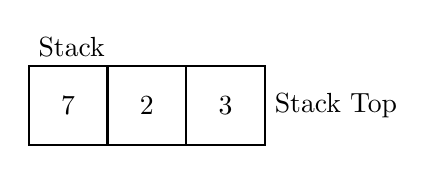
\begin{tikzpicture}
        \draw [thick] (0,0) rectangle (1,1);
        \draw [thick] (1,0) rectangle (2,1);
        \draw [thick] (2,0) rectangle (3,1);
        \node at (0.5, 0.5) {7};
        \node at (1.5, 0.5) {2};
        \node at (2.5, 0.5) {3};
        \node [right] at (3, 0.5) {Stack Top};
        \node [above right] at (0, 1) {Stack};
    \end{tikzpicture}
    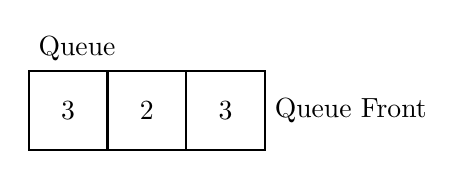
\begin{tikzpicture}
        \draw [thick] (0,0) rectangle (1,1);
        \draw [thick] (1,0) rectangle (2,1);
        \draw [thick] (2,0) rectangle (3,1);
        \node at (0.5, 0.5) {3};
        \node at (1.5, 0.5) {2};
        \node at (2.5, 0.5) {3};
        \node [right] at (3, 0.5) {Queue Front};
        \node [above right] at (0, 1) {Queue};
    \end{tikzpicture}
    \subsection{}
    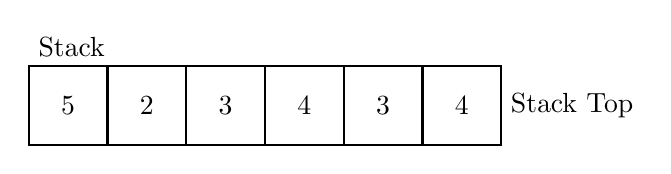
\begin{tikzpicture}
        \draw [thick] (0,0) rectangle (1,1);
        \draw [thick] (1,0) rectangle (2,1);
        \draw [thick] (2,0) rectangle (3,1);
        \draw [thick] (3,0) rectangle (4,1);
        \draw [thick] (4,0) rectangle (5,1);
        \draw [thick] (5,0) rectangle (6,1);
        \node at (0.5, 0.5) {5};
        \node at (1.5, 0.5) {2};
        \node at (2.5, 0.5) {3};
        \node at (3.5, 0.5) {4};
        \node at (4.5, 0.5) {3};
        \node at (5.5, 0.5) {4};
        \node [above right] at (0, 1) {Stack};
        \node [right] at (6, 0.5) {Stack Top};
    \end{tikzpicture}
    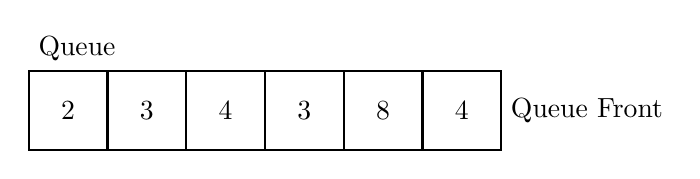
\begin{tikzpicture}
        \draw [thick] (0,0) rectangle (1,1);
        \draw [thick] (1,0) rectangle (2,1);
        \draw [thick] (2,0) rectangle (3,1);
        \draw [thick] (3,0) rectangle (4,1);
        \draw [thick] (4,0) rectangle (5,1);
        \draw [thick] (5,0) rectangle (6,1);
        \node at (0.5, 0.5) {2};
        \node at (1.5, 0.5) {3};
        \node at (2.5, 0.5) {4};
        \node at (3.5, 0.5) {3};
        \node at (4.5, 0.5) {8};
        \node at (5.5, 0.5) {4};
        \node [above right] at (0, 1) {Queue};
        \node [right] at (6, 0.5) {Queue Front};
    \end{tikzpicture}
    \subsection{}
    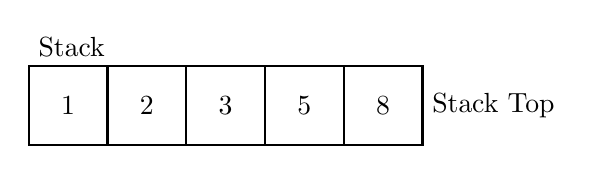
\begin{tikzpicture}
        \draw [thick] (0,0) rectangle (1,1);
        \draw [thick] (1,0) rectangle (2,1);
        \draw [thick] (2,0) rectangle (3,1);
        \draw [thick] (3,0) rectangle (4,1);
        \draw [thick] (4,0) rectangle (5,1);
        \node at (0.5, 0.5) {1};
        \node at (1.5, 0.5) {2};
        \node at (2.5, 0.5) {3};
        \node at (3.5, 0.5) {5};
        \node at (4.5, 0.5) {8};
        \node [above right] at (0, 1) {Stack};
        \node [right] at (5, 0.5) {Stack Top};
    \end{tikzpicture}
    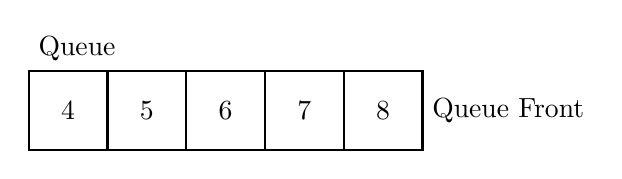
\begin{tikzpicture}
        \draw [thick] (0,0) rectangle (1,1);
        \draw [thick] (1,0) rectangle (2,1);
        \draw [thick] (2,0) rectangle (3,1);
        \draw [thick] (3,0) rectangle (4,1);
        \draw [thick] (4,0) rectangle (5,1);
        \node at (0.5, 0.5) {4};
        \node at (1.5, 0.5) {5};
        \node at (2.5, 0.5) {6};
        \node at (3.5, 0.5) {7};
        \node at (4.5, 0.5) {8};
        \node [above right] at (0, 1) {Queue};
        \node [right] at (5, 0.5) {Queue Front};
    \end{tikzpicture}
    \section{}
        \subsection{}
        $O(a + b + c)$

        Always returns $0$.
        \subsection{}
        $O(1)$

        Calculates n factorial.
        \subsection{}
        $O(1)$

        Will always return n.
    \section{}
    $T1(n) \leq cf(n)$ and $T2(n) \leq cg(n)$, therefore $T1(n) + T2(n) \leq cf(n) + cg(n) \Rightarrow T1(n) + T2(n) \leq c(f(n) + g(n))$ so by the definition of Big O, $T1(n) + T2(n) = O(f(n) + g(n))$ 
\end{document}